\documentclass[12pt]{report}

\usepackage[a4paper]{geometry}
\geometry{left=2.5cm,right=2.5cm,top=2.5cm,bottom=2.5cm, a4paper}
\usepackage[utf8]{inputenc}
\usepackage{amsmath}
\usepackage{amsthm}
\usepackage{amssymb}
\usepackage{ulem}
\usepackage{graphicx}
\usepackage{caption}
\graphicspath{}
\usepackage[document]{ragged2e}
\usepackage{setspace}
\usepackage{tabularx}
\usepackage[slovene]{babel}
\usepackage{gensymb}
\usepackage{siunitx}
\usepackage{pdfrender,xcolor}
\usepackage{hyperref}
\usepackage{xurl}
\usepackage{float}
\usepackage{titlesec}
\usepackage{physics}

\newfloat{slika}{htbp}{loc}
\floatname{slika}{Slika}

\newfloat{tabela}{htbp}{loc}
\floatname{tabela}{Tabela}

\title{
  
\includegraphics[width=0.4\textwidth]{fmf_logo}\\
  {\small Oddelek za fiziko} \\
  {Akustični resonator}\\
  {\small Poročilo pri fizikalnem praktikumu III}\\

}
\date{}
\author{ Kristofer Č. Povšič \\[5 cm]
 \small  Mentor: Jelena Vesić\\
}

\titleformat{\chapter}[hang]{\Huge\bfseries}{\thechapter{. }}{0pt}{\Huge\bfseries}

\setlength\parindent{0pt}

\begin{document}

\setcounter{page}{2}

\maketitle

\chapter*{Uvod}

Proste oscilacije pri določenih frekvencah, ki se pojavijo v zaprtem omejenem prostoru, imenujemo lastne frekvence. Z uporabo Newtonovega zakona za kontinuum, kontinuitetne enačbe, enačbe za adiabatne stisljivosti in enačbo za hitrosti zvoka dobimo sledečo enačbo \ref{eq:1}:

\begin{equation}\label{eq:1}
  \laplacian{\delta p} = \frac{1}{c^2} \frac{\partial^2 \delta p}{\partial t^2}
\end{equation}

kjer je $\delta p$ odmik tlaka od ravnovesne lege, $c$ hitrost zvoka, $t$ pa čas. 

Pravokotnih odmikov v smeri $\vec{n}$ na steno ni, kar nam služi kot robni pogoj. Z uporabo nastavka in kosinusov zadostimo robni pogoj. Določimo nastavek: 

\begin{equation}\label{eq:nast}
  \begin{aligned}
    \vec{r} = (x, y, z) \\  
    p(\vec{r}, t) = p(\vec{r})cos(\omega t + \phi) \\
    p(\vec{r}) = p_0 \cos (k_x x) \cos (k_y y) \cos (k_z z)
  \end{aligned}
\end{equation}


Nastavek \ref{eq:nast} uporabimo v enačbi \ref{eq:1} in dobimo zvezo med kotno frekvenco $\omega$ in valovnim vektorjem $\vec{k} = (k_x, k_y, k_z)$:
\begin{equation}
  \frac{\omega^2}{c^2} = k_x^2 + k_y^2 + k_z^2
\end{equation}

Z upoštevanjem robnih pogojev na kvadru s stranicami A, B in C dobimo 

\begin{equation}
  \begin{aligned}
    k_x = \frac{n_x \pi}{A}\\
    k_y = \frac{n_y \pi}{B}\\
    k_z = \frac{n_z \pi}{C}\\
  \end{aligned}
\end{equation}


kjer so $n_x$, $n_y$, $n_z$ $\in \mathbb{Z} \cup \{0\}$. Kotne frekvence lastnih valovanj so tako

\begin{equation}\label{eq:om}
  \omega = c \pi \sqrt{\left(\frac{n_x}{A}^2\right) + \left(\frac{n_y}{B}^2\right) + \left(\frac{n_z}{C}^2\right)}
\end{equation}


\chapter*{Naloga}

\begin{itemize}
  \item Izračunaj najnižje resonančne frekvence akustičnega resonatorja za $n_i$ od 0 do 3 in dobljene frekvence (manjše od $1000Hz$) v tabeli razvrsti po velikosti skupaj s pripadajočimi vrednostmi $n_i$. V tabeli pusti še dva prazna stolpca za izmerjene frekvence in amplitude. 
  \item Izmeri resonančni odziv akustičnega resonatorja v območju od $200$ do $1000Hz$ in ga nariši na ustrezen graf.
  \item Izmeri odvisnost signala od položaja mikrofona v škatli in za osnovno in še nekatere višje resonance. Izberi si take frekvence, da bodo odvisnosti $p(\vec{r})$ različne (recimo za $n_x$ od 0 do 3). 
  \item Primerjaj izmerjene in izračunane frekvence in na ta način določi, kateremu nihajnemu načinu pripadajo izmerjene resonance. Frekvence maksimumov in ustrezne amplitude vnesi v pripravljeno tabelo. 
  \item Iz prvih treh resonanc izračunaj hitrost zvoka. 
  \item Oceni razpolovno širino prvih treh resonančnih črt in še katere, ki je dovolj ločena od ostalih. 
\end{itemize}


\begingroup
\let\clearpage\relax

\chapter*{Potrebščine}
\begin{itemize}
  \item Akustični resonator - zaboj iz vezanih in ivernih plošč z debelimi dušenimi stenami, notranje dimenzija so $A \times B \times C = 56.7\text{cm}\times 38.5\text{cm} \times 24.0 \text{cm}$ (nedoločnost $\pm 0.1$cm) z odstranljivim pokrovom
  \item prenosnik opremljen s programom AkRes in zunanjo zvočno kartico, ki podpira 44.1kHz Mono-Duplex način predvajanja in sprejemanja zvoka
  \item zvočnik, pritrjen na steno resonatorja blizu vogala in povezan preko ojačevalca na izhod zunanje zvočne kartice 
  \item premični mikrofon povezan na vhod zunanje zvočne kartice. 
\end{itemize}

\chapter*{Navodilo}

Meritev opravimo tako, da merimo zvočno jakost v resonatorju z mikrofonom, pri čemer vzbujamo valovanje z zvočnikom, na katerega priključimo izvor s konstantno amplitudo napetosti ali toka. 

Meritev izmerimo s pomočjo programa, ki shrani 4 vrednosti: generirano frekvenco, amplitudo, standardno deviacijo amplitude in amplitudo odziva s pomočjo t.i. sinhrone detekcije (ang. lock-in detection). Tako zvočni profil kot resonančni odziv izmerimo s pomočjo tega programa. 

\endgroup


\chapter*{Meritve in izračunane vrednosti}

Izmerjene in izračunane so bile naslednje vrednosti

\[
\begin{array}{|c|c|c|c|c|c|} \hline
  \vec{n} & \nu_{izr}[Hz] & \nu_{izm}[Hz] & A & \sigma_A & A_{\nu} \\ \hline
  (1, 0, 0) & 299.82 & 308 & 0.53 & 0.32 & 0.43 \\ \hline
  (2, 0, 0) & 599.65 & 607 & 0.93 & 0.62 & 0.88 \\ \hline
  (3, 0, 0) & 899.47 & 911 & 0.71 & 0.42 & 0.62 \\ \hline
  (0, 1, 0) & 441.56 & 450 & 0.72 & 0.45 & 0.64\\ \hline
\end{array}
\]

\section*{Resonančni odziv}

\begin{slika}[H]
  \centering
  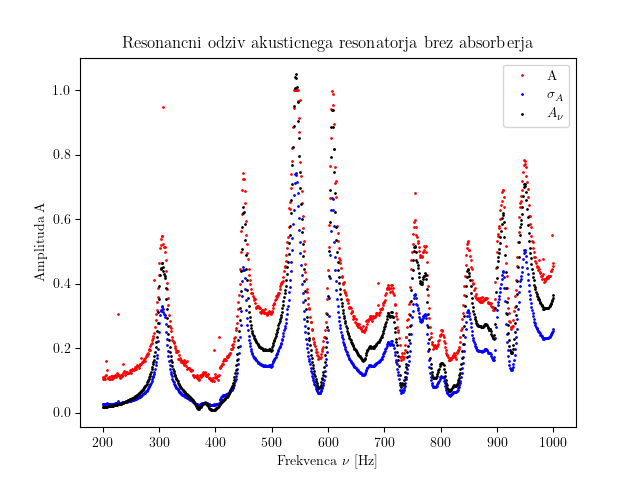
\includegraphics{01Neduseno}
  \caption{\small Graf prikazuje resonančni odziv akustičnega resonatorja brez absorberja za frekvence med $200$ in $1000Hz$. }
  \label{fig:odz_n}
\end{slika}

\begin{slika}[H]
  \centering
  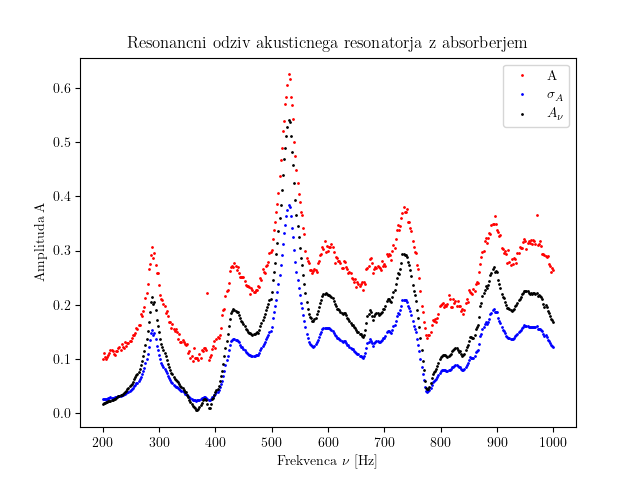
\includegraphics{02Duseno}
  \caption{\small Graf prikazuje resonančni odziv akustičnega resonatorja z absorberjem (črno blago) za frekvence med $200$ in $1000Hz$. }
  \label{fig:odz_d}
\end{slika}

Če primerjamo grafa \ref{fig:odz_n} in \ref{fig:odz_d} vidimo, da ima graf \ref{fig:odz_d} manjšo amplitudo in bolj sploščene vrhove pri resonancah.

\section*{Zvočni profil}

\begin{figure}[H]
  \centering
  \begin{minipage}[b]{0.75\textwidth}
    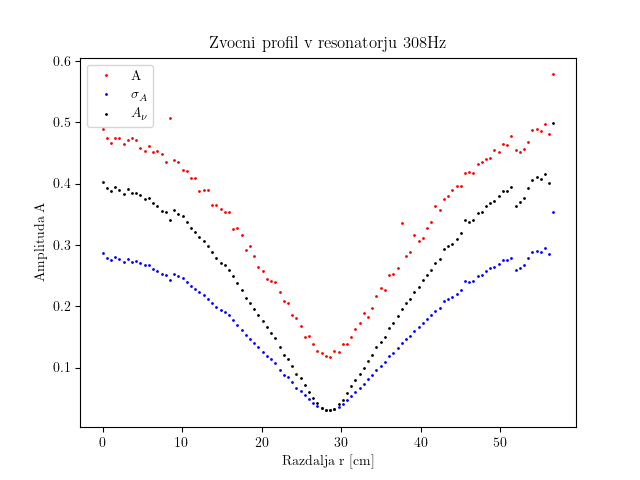
\includegraphics[width=1\textwidth]{03308Hz}
    \captionof{slika}{\small Graf prikazuje zvočni profil v resonatorju pri frekvenci $308Hz$}
    \label{fig:308Hz}
  \end{minipage}
  \begin{minipage}[b]{0.75\textwidth}
    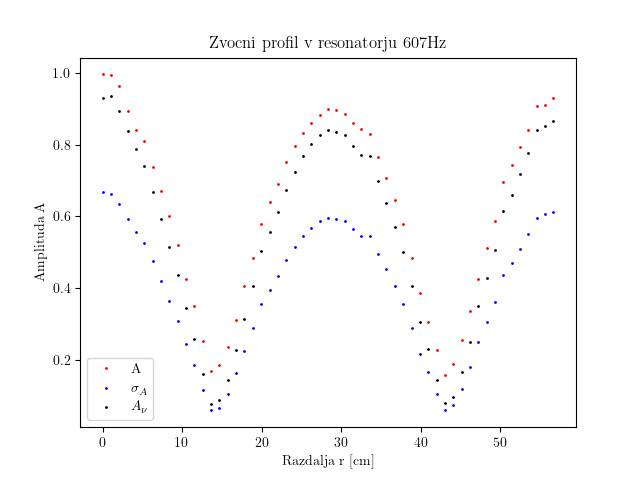
\includegraphics[width=1\textwidth]{04607Hz}
    \captionof{slika}{\small Graf prikazuje zvočni profil v resonatorju pri frekvenci $607Hz$}
    \label{fig:607Hz}
  \end{minipage}
\end{figure}

\begin{figure}[H]
  \centering
  \begin{minipage}[b]{0.75\textwidth}
    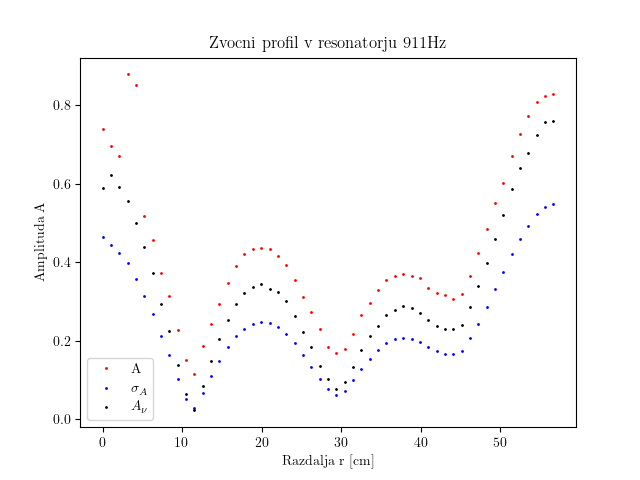
\includegraphics[width=1\textwidth]{05911Hz}
    \captionof{slika}{\small Graf prikazuje zvočni profil v resonatorju pri frekvenci $911Hz$}
    \label{fig:911Hz}
  \end{minipage}
  \begin{minipage}[b]{0.75\textwidth}
    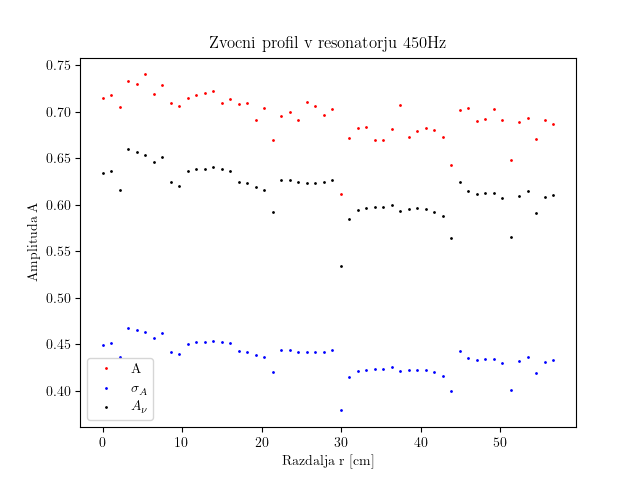
\includegraphics[width=1\textwidth]{06450Hz}
    \captionof{slika}{\small Graf prikazuje zvočni profil v resonatorju pri frekvenci $450Hz$}
    \label{fig:450Hz}
  \end{minipage}
\end{figure}

Na grafih opazimo, da amplituda v odvisnosti od frekvence pade ponekod na skoraj 0. Naš akustični resonator je v zaprta piščal, ki smo jo obravnavali pri predavanjih Klasične fizike in tam, kjer je amplituda skoraj 0, je t.i. vozel. 

Na grafu \ref{fig:450Hz} ni vidnega vozla, saj je zvočni profil narejeno v x-smeri (po daljši stranici, horizontalno). Da bi se pri tej resonančni krivulji dobili podoben graf ostalim, bi moral zvočni profil narediti po drugi dimenziji - v globino ali pa v širino.

\section*{Hitrost zvoka in ocena razpolovne širine}

Iz formule \ref{eq:om} izrazimo hitrost in dobimo sledečo enačbo: 

\begin{equation}
  c = \frac{2\nu}{\sqrt{\left(\frac{n_x}{A}\right)^2 + \left(\frac{n_y}{B}\right)^2 \left(\frac{n_z}{C}\right)^2}}
\end{equation}

\[
  \begin{array}{|c|c|c|} \hline
    \nu [Hz] & c [m/s] & napaka [m/s] \\ \hline
    308 &  349.3 & 0.6 \\ \hline
    607 & 344.2 & 0.6 \\ \hline
    911 & 344.4 & 0.6\\ \hline
  \end{array}  
\]

Izračunamo povprečno hitrost zvoka, ki je $c=345.9m/s \pm 3.3m/s$.

Pri resonančni črti izračunamo polovično vrednost maksimalne amplitude in pri tej vrednosti pogledamo, kako širok je val, delimo z 2 in s tem dobimo razpolovno širino resonančnih črt. 

\[
  \begin{array}{|c|c|}\hline
    \nu[Hz] & \Delta \nu \pm 1 [Hz] \\ \hline
    308 & 13.5  \\ \hline
    450 & 11.5 \\ \hline
    542 & 16 \\ \hline
    607 & 9\\ \hline
  \end{array}
\]

\end{document}